\documentclass[aspectratio=169]{beamer}
\usepackage[utf8]{inputenc}
\usepackage[T5]{fontenc}
\usepackage[vietnamese]{babel}
\usepackage{graphicx}
\usepackage{hyperref}
\usepackage{lmodern}

% Theme
\usetheme{Madrid}
\usecolortheme{whale}

% Metadata
\title[AI trong NN]{Ứng dụng AI trong Nông nghiệp}
\subtitle{Chương 12: Nông nghiệp chính xác}
\author{Giảng viên}
\institute{Đại học Đông Á}
\date{\today}

\begin{document}

\begin{frame}
    \titlepage
\end{frame}

\begin{frame}{Nội dung chính}
    \tableofcontents
\end{frame}

\section{Giới thiệu chung}
\begin{frame}{Giới thiệu chung}
    \begin{itemize}
        \item Ngành nông nghiệp đóng vai trò quan trọng trong nền kinh tế, đặc biệt ở các nước đang phát triển (ví dụ: Ấn Độ).
        \item Mặc dù diện tích đất canh tác giảm, nhưng số lượng dân số và nhu cầu lương thực lại tăng lên.
        \item \textbf{Nông nghiệp chính xác} (Precision Agriculture/Farming) ra đời nhằm:
        \begin{itemize}
            \item \textbf{Làm đúng việc, đúng cách, đúng nơi và đúng thời điểm.}
            \item Thu thập, xử lý và phân tích dữ liệu không gian, thời gian.
            \item Hỗ trợ quyết định quản lý nhằm nâng cao hiệu quả, năng suất, chất lượng và lợi nhuận.
        \end{itemize}
    \end{itemize}
\end{frame}

\section{Khái niệm Nông nghiệp chính xác}
\begin{frame}{Khái niệm Nông nghiệp chính xác}
    \begin{block}{Hệ thống Nông nghiệp Chính xác (PFS)}
        Tập trung vào nhận diện sự biến đổi theo không gian và thời gian trong quá trình phát triển của cây trồng để quản lý, từ đó tăng năng suất và giảm rủi ro môi trường.
    \end{block}
    
    \vspace{0.3cm}
    Một tập hợp các công nghệ cho phép:
    \begin{itemize}
        \item Thu thập dữ liệu ở quy mô và thời điểm thích hợp.
        \item Diễn giải và phân tích dữ liệu để hỗ trợ lựa chọn quản lý.
        \item Áp dụng phản ứng quản lý đúng mức độ và đúng thời điểm.
    \end{itemize}
\end{frame}

\section{Lợi ích}
\begin{frame}{Lợi ích của Nông nghiệp chính xác}
    \begin{itemize}
        \item \textbf{Tăng tổng sản lượng}: Áp dụng đúng loại/liều lượng phân bón, thuốc bảo vệ thực vật giúp cây sinh trưởng tối ưu.
        \item \textbf{Cải thiện hiệu quả}: Tiết kiệm thời gian và sức lao động (ví dụ: máy móc giúp trồng 1ha ngô chỉ trong 2 giờ).
        \item \textbf{Giảm chi phí sản xuất}: Bón phân đúng thời điểm và lượng cần thiết giúp tiết kiệm đầu vào.
        \item \textbf{Ra quyết định dựa trên dữ liệu}: Thu thập thông tin đáng tin cậy để gieo hạt, tưới tiêu, thoát nước hợp lý.
        \item \textbf{Bảo vệ môi trường}: Tránh dư thừa hóa chất ngấm vào đất và nguồn nước.
        \item \textbf{Tích lũy tri thức}: Lưu trữ dữ liệu lâu dài hỗ trợ nông dân cải thiện kỹ năng quản lý.
    \end{itemize}
\end{frame}

\section{Các bước cơ bản}
\begin{frame}{Các bước cơ bản trong Nông nghiệp chính xác (1/2)}
    \begin{enumerate}
        \item \textbf{Đánh giá sự biến đổi}:
        \begin{itemize}
            \item "Không thể quản lý những gì bạn không biết".
            \item Cần đánh giá sự biến đổi theo không gian (các khu vực đất khác nhau) và thời gian (các mùa sinh trưởng).
            \item Sự trợ giúp của AI (Computer Vision, Big Data) giúp thu thập dữ liệu nhanh và chính xác hơn.
        \end{itemize}
        \vspace{0.3cm}
        \item \textbf{Quản lý sự biến đổi}:
        \begin{itemize}
            \item Điều chỉnh các yếu tố đầu vào (nước, phân bón) phù hợp với đặc thù từng địa điểm.
            \item Ghi nhớ tọa độ (GPS) để lấy mẫu và theo dõi chính xác.
            \item Sử dụng các Bot/Drone để giám sát đồng ruộng diện rộng.
        \end{itemize}
    \end{enumerate}
\end{frame}

\begin{frame}{Các bước cơ bản trong Nông nghiệp chính xác (2/2)}
    \begin{enumerate}
        \setcounter{enumi}{2}
        \item \textbf{Đánh giá (Evaluation)}:
        \begin{itemize}
            \item Phân tích lợi ích kinh tế thu được so với chi phí áp dụng công nghệ.
            \item Đánh giá tác động môi trường (giảm thoái hóa đất, giảm ô nhiễm).
        \end{itemize}
        \vspace{0.3cm}
        \item \textbf{Hành động cuối cùng}:
        \begin{itemize}
            \item Ứng dụng công nghệ chuyển giao vào thực tiễn canh tác (Chuyển giao công nghệ).
            \item Kết nối các trang trại thông qua cơ sở hạ tầng mạng.
        \end{itemize}
    \end{enumerate}
\end{frame}

\section{Triển khai AI trong NN Chính xác}
\begin{frame}{Triển khai Trí tuệ nhân tạo trong Nông nghiệp chính xác}
    AI được áp dụng thông qua quy trình 3 bước cốt lõi:
    \begin{figure}[h]
        \centering
        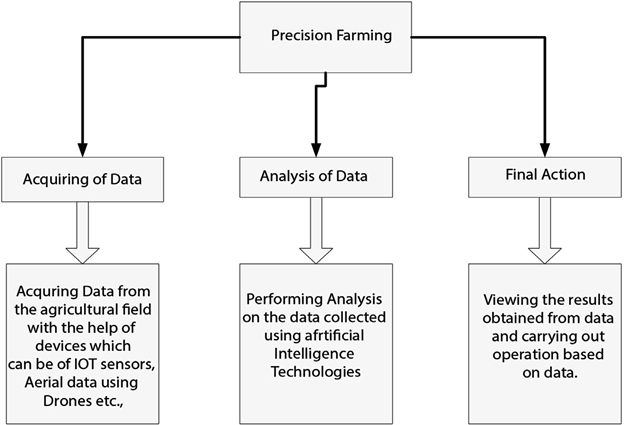
\includegraphics[width=0.6\textwidth]{images/chap12_p4_1.png}
        \caption{Sơ đồ quy trình triển khai AI trong Nông nghiệp chính xác}
    \end{figure}
\end{frame}

\begin{frame}{Bước 1: Thu thập dữ liệu}
    \begin{itemize}
        \item \textbf{IoT trong nông nghiệp}: Các cảm biến quang phổ, cảm biến độ ẩm giúp đo lượng N-P-K và độ ẩm đất. Giảm lãng phí phân bón lên đến 30\%.
        \item \textbf{Drone và Hình ảnh vệ tinh}: 
        \begin{itemize}
            \item Drone chụp ảnh độ phân giải cao cận cảnh.
            \item Vệ tinh chụp toàn cảnh rộng lớn.
            \item Kết hợp tạo bản đồ đường đồng mức, đánh giá dòng chảy, dự báo năng suất.
        \end{itemize}
        \item \textbf{Robot (Agricultural Bots)}: 
        \begin{itemize}
            \item Máy kéo tự lái lập trình bằng GPS.
            \item Robot nhận diện và nhổ cỏ dại hoặc hái quả tự động.
        \end{itemize}
    \end{itemize}
\end{frame}

\begin{frame}{Bước 2 \& Bước 3: Phân tích dữ liệu và Hành động}
    \textbf{Bước 2: Phân tích dữ liệu}
    \begin{itemize}
        \item Dữ liệu khổng lồ từ Bước 1 được phân tích bằng Học máy (ML), Học sâu (DL), và Thị giác máy tính để tìm ra các mẫu quy luật có giá trị.
    \end{itemize}
    \vspace{0.3cm}
    \textbf{Bước 3: Hành động cuối cùng (Ứng dụng cụ thể)}
    \begin{itemize}
        \item \textbf{Bot nông nghiệp}: Xử lý hạt giống, thu hoạch.
        \item \textbf{Chọn giống}: Dự đoán gen chịu hạn, kháng bệnh dựa trên phân tích thống kê hàng thập kỷ dữ liệu.
        \item \textbf{Nhận dạng loài / cỏ dại}: Phân loại hình thái lá qua hình ảnh để phun thuốc chọn lọc, tiết kiệm hóa chất.
    \end{itemize}
\end{frame}

\section{Ứng dụng cụ thể}
\begin{frame}{Các ứng dụng quản lý bằng AI}
    \begin{itemize}
        \item \textbf{Dự đoán năng suất}: Không chỉ dựa vào lịch sử, AI khớp nối thời tiết, thị trường và đa chiều dữ liệu để tối ưu hóa lợi nhuận.
        \item \textbf{Dự báo và phát hiện bệnh}: Phân tích viễn thám giúp giám sát hàng nghìn hecta, phát hiện dịch hạch ngay lập tức thay vì đi tuần tra bộ.
        \item \textbf{Quản lý đất đai và nguồn nước}:
        \begin{itemize}
            \item Phân tích nhiệt độ, sự bốc hơi đất.
            \item Tưới tiêu thông minh dự báo theo điểm sương và sự bốc hơi hàng tuần.
        \end{itemize}
        \item \textbf{Chăn nuôi}: Ước tính và dự báo trọng lượng gia súc trước ngày giết mổ để thay đổi chế độ dinh dưỡng tối ưu.
    \end{itemize}
\end{frame}

\section{Thách thức \& Hạn chế}
\begin{frame}{Thách thức trong việc áp dụng AI (Phần 1)}
    Dù mang lại lợi ích to lớn, Nông nghiệp chính xác ở các nước đang phát triển (như Ấn Độ, Việt Nam) gặp nhiều rào cản:
    \begin{itemize}
        \item \textbf{Quy mô đồng ruộng nhỏ manh mún}: Khó áp dụng máy móc cơ giới cỡ lớn.
        \item \textbf{Chi phí phần cứng cao}: Drone, cảm biến quang phổ, trạm thu phát sóng có chi phí bảo trì và vận hành đắt đỏ.
        \item \textbf{Thiếu kỹ năng địa phương}: Tỷ lệ nông dân biết sử dụng công nghệ số còn hạn chế.
        \item \textbf{Biến đổi thời tiết}: Mưa bão, ô nhiễm không khí làm nhiễu sóng cảm biến và che khuất camera vệ tinh.
    \end{itemize}
\end{frame}

\begin{frame}{Thách thức trong việc áp dụng AI (Phần 2)}
    \begin{itemize}
        \item \textbf{Quản lý dữ liệu dư thừa (Big Data)}:
        \begin{itemize}
            \item Khối lượng ảnh và thông số tạo ra mỗi ngày rất lớn, đòi hỏi Cloud Server cấu hình cao.
            \item Rủi ro bảo mật dữ liệu bị hacker tấn công/làm sai lệch.
        \end{itemize}
        \item \textbf{Hạ tầng kết nối}: Cần mạng 5G phủ sóng diện rộng tại các vùng nông thôn để thiết bị IoT giao tiếp theo thời gian thực (Real-time).
        \item \textbf{Khả năng tương tác}: Các thiết bị từ nhiều hãng khác nhau chưa có chuẩn kết nối chung, gây khó khăn khi đồng bộ dữ liệu.
    \end{itemize}
\end{frame}

\section{Tóm tắt}
\begin{frame}{Tóm tắt}
    \begin{block}{Nông nghiệp chính xác}
        Là cách tiếp cận hiện đại sử dụng IoT, AI, Cloud Computing, và Drone để tối ưu hóa nguồn lực (nước, phân bón, thuốc trừ sâu) dựa trên sự biến đổi thực tế của đất đai và cây trồng.
    \end{block}
    \begin{block}{Triển vọng}
        Dù còn nhiều thách thức về chi phí hạ tầng và kỹ năng của người nông dân, AI là giải pháp bắt buộc để hướng tới một nền nông nghiệp cạnh tranh, năng suất vượt trội và bền vững với môi trường.
    \end{block}
\end{frame}

\begin{frame}
    \centering \Huge \textbf{Xin Cảm Ơn!}
\end{frame}

\end{document}
